\documentclass[border=3pt]{standalone}
\usepackage{amsmath,amssymb,xcolor,fontspec,tikz}
\usetikzlibrary{arrows.meta,angles,quotes,positioning}
\setmainfont{NimbusRoman-Regular.otf}[Path=/usr/share/fonts/opentype/urw-base35/,BoldFont=NimbusRoman-Bold.otf,ItalicFont=NimbusRoman-Italic.otf,BoldItalicFont=NimbusRoman-BoldItalic.otf]
\definecolor{fg}{HTML}{EEF2F6}\definecolor{bg}{HTML}{0B1015}
\definecolor{yel}{HTML}{FFD45C}\definecolor{cya}{HTML}{70DCF5}

\begin{document}
\color{fg}
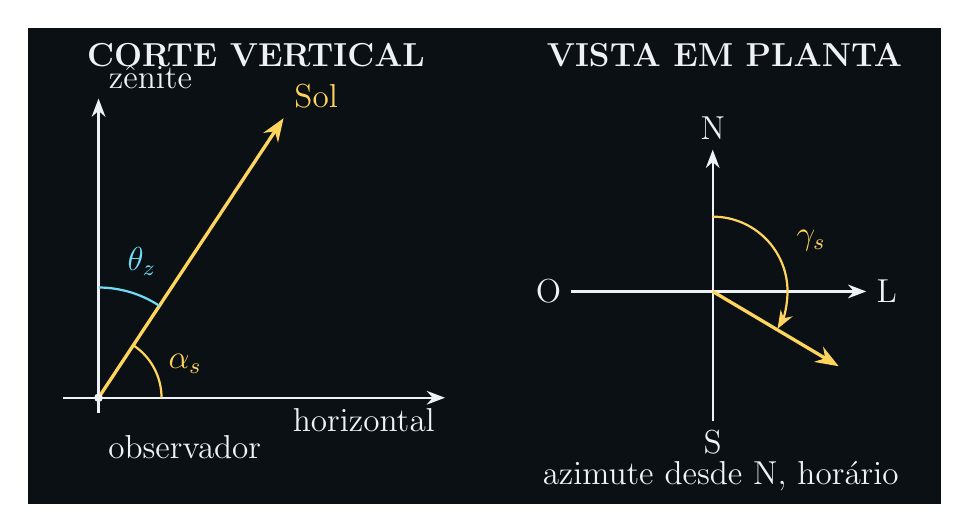
\begin{tikzpicture}[x=1cm,y=1cm,>=Stealth,font=\large]
\path[fill=bg](-.9,-1.35)rectangle(10.7,4.7);
\node[fg,font=\bfseries\large] at (2,4.35){CORTE VERTICAL};
\draw[fg,->,thick](-.45,0)--(4.4,0)node[below left]{horizontal};
\draw[fg,->,thick](0,-.2)--(0,3.8)node[above right]{zênite};
\draw[yel,->,very thick](0,0)--(2.35,3.55)node[above right]{Sol};
\draw[yel,thick](.8,0)arc[start angle=0,end angle=56.5,radius=.8];
\node[yel] at (1.1,.43){$\alpha_s$};
\draw[cya,thick](0,1.4)arc[start angle=90,end angle=56.5,radius=1.4];
\node[cya] at (.55,1.73){$\theta_z$};
\fill[fg](0,0)circle(.055);\node[fg,below right]at(0,-.35){observador};
\node[fg,font=\bfseries\large] at (7.95,4.35){VISTA EM PLANTA};
\begin{scope}[shift={(7.8,1.35)}]
\draw[fg,->,thick](0,-1.65)--(0,1.8)node[above]{N};
\draw[fg,->,thick](-1.8,0)--(1.95,0)node[right]{L};
\node[fg,below]at(0,-1.65){S};\node[fg,left]at(-1.8,0){O};
\draw[yel,->,very thick](0,0)--(1.6,-.95);
\draw[yel,->,thick](0,.95)arc[start angle=90,end angle=-30,radius=.95];
\node[yel]at(1.25,.65){$\gamma_s$};
\end{scope}
\node[fg] at (7.9,-1.0){azimute desde N, horário};
\end{tikzpicture}
\end{document}
